\documentclass[12pt,article]{article}
\usepackage{fullpage}
\usepackage[top=2cm, bottom=4.5cm, left=2cm, right=2cm]{geometry}
\usepackage{amsmath,amsthm,amsfonts,amssymb,amscd}
\usepackage{lastpage}
\usepackage{enumerate}
\usepackage{fancyhdr}
\usepackage{mathrsfs}
\usepackage{xcolor}
\usepackage{graphicx}
\usepackage{listings}
\usepackage{hyperref}
\usepackage{mdframed}
\usepackage{changepage}   % for the adjustwidth environment
\usepackage{forest} 
\usepackage{tikz}   % For graph

\usepackage{float}  % To inforce inserting images at the right place
\restylefloat{table}

\usepackage[center]{caption}

\usepackage{caption}
\usepackage{subcaption}

\usepackage{algorithm}
\usepackage{algpseudocode}
\usepackage{graphicx,txfonts}


% For recursive formulation, adapted from https://tex.stackexchange.com/questions/580333/typing-sequences-recursively-in-overleaf
\usepackage{mathtools}
\makeatletter
\newcases{centercases}{\quad}
  {\hfil$\m@th\displaystyle{##}$\hfil}
  {$\m@th\displaystyle{##}$\hfil}{\lbrace}{.}
\makeatother

\newcommand{\Tau}{\mathrm{T}}
\newcommand{\heart}{\ensuremath\varheartsuit}


% For matrix
\def\horzbar{\text{magic}}

\hypersetup{%
  colorlinks=true,
  linkcolor=blue,
  linkbordercolor={0 0 1}
}

\setlength{\parindent}{0.0in}
\setlength{\parskip}{0.05in}

\newcommand\projnumber{2}
\newcommand\course{CS534}
\newcommand\OSUID{934370552}
\newcommand\Email{buivy@oregonstate.edu}
\newcommand\Name{Vy Bui}
\newcommand\tab[1][1cm]{\hspace*{#1}}

\pagestyle{fancyplain}
\headheight 35pt
\lhead{Homework \projnumber}
\rhead{Feb 8, 2023}
\lfoot{}
\cfoot{}
\rfoot{\small\thepage}
\headsep 1.5em

\newenvironment{task}[2][Task]
    { \begin{mdframed}[backgroundcolor=gray!20] \textbf{#1 #2} \\}
    {  \end{mdframed}}
   

% Make Rightarrow with superscript
% \makeatletter
% \newcommand{\xRightarrow}[2][]{\ext@arrow 0359\Rightarrowfill@{#1}{#2}}
% \makeatother

\begin{document}

\begin{titlepage}
    \begin{center}
        \vspace*{4cm}

        \textbf{\Large AI539 - Natural Language Processing with Deep Learning}

        \vspace{0.5cm}
 
        \textbf{ Homework 2 Report}

        \textbf{ Recurrent Neural Networks and Sentence Representations }
 
        \vspace{1cm}

        Author: Vy Bui

        OSUID: 934370552

        \vspace{1cm}

        Instructor: Professor Stefan Lee
        \vfill
             
        \vspace{0.8cm}
      
             
        The School of Electrical Engineering and Computer Science\\
        Oregon State University\\
             
    \end{center}
\end{titlepage}


%==============================================================================%
\newpage
\begin{task}{1.1} 
Manually find weights and biases for the univariate LSTM defined above such that the final hidden state will be greater than or equal to 0.5 for odd parity strings and less than 0.5 for even parity. The parameters you must provide values for are $w_{ix}$, $w_{ih}$, $b_i$, $w_{fx}$, $w_{fh}$, $b_f$, $w_{ox}$, $w_{oh}$, $b_o$, $w_{gx}$, $w_{gh}$, $b_g$ and are all scalars. The LSTM will take one bit of the string (0 or 1) as input $x$ at each time step. A tester is set up in \texttt{univariate\_tester.py} where you can enter your weights and check performance. \\[5pt]

\emph{Hints: Some of the weights will likely be zero. Others may be large. Scale matters, larger weights will saturate the activation functions. Also note that \texttt{A XOR B} can be written as \texttt{(A OR B) AND (A NAND B)}. Work backwards and try to find where this sort of two-term structure could be implemented.} 
\end{task}

%==============================================================================%
\newpage
\begin{task}{2.1} 
Implement the \texttt{ParityLSTM} class in \texttt{driver\_parity.py}. Your model's \texttt{forward} function should process the batch of binary input strings and output a $B \times 2$ tensor $y$ where $y_{b,0}$ is the score for the $b^{th}$ element of the batch having an even parity and $y_{b,1}$ for odd parity. You may use any PyTorch-defined LSTM functions. Larger hidden state sizes will make for easier training in my experiments. Running \texttt{driver\_parity.py} will train your model and output per-epoch training loss and accuracy. A correctly-implemented model should approach 100\% accuracy on the training set. In your write-up for this question, describe any architectural choices you made.\\[5pt]

\emph{Hint: Efficiently processing batches with variable input lengths requires some bookkeeping or else the LSTM will continue to process the padding for shorter sequences along with the content of longer ones. See pack\_padded\_sequence and pad\_packed\_sequence documentation in PyTorch.}
\end{task}

The model takes one input feature at a time, including one layer of LSTM with 64 hidden units. The final states of these units are fed to a 2 back-to-back Linear layers with the shape of $128 \times 128$ and $128 \times 2$, respectively. Their outputs then go to a sigmoid function to generate probabilities for even and odd parity.

Various learning rates were examined and the best learning rate appeared to be 0.0005. The model's training process is depicted by the Figure \ref{fig:lstm128-training}. It took around 18000 epochs to drive the train accuracy up to 1.

\begin{figure}[H]
\centering
\begin{subfigure}{.5\textwidth}
    \centering
    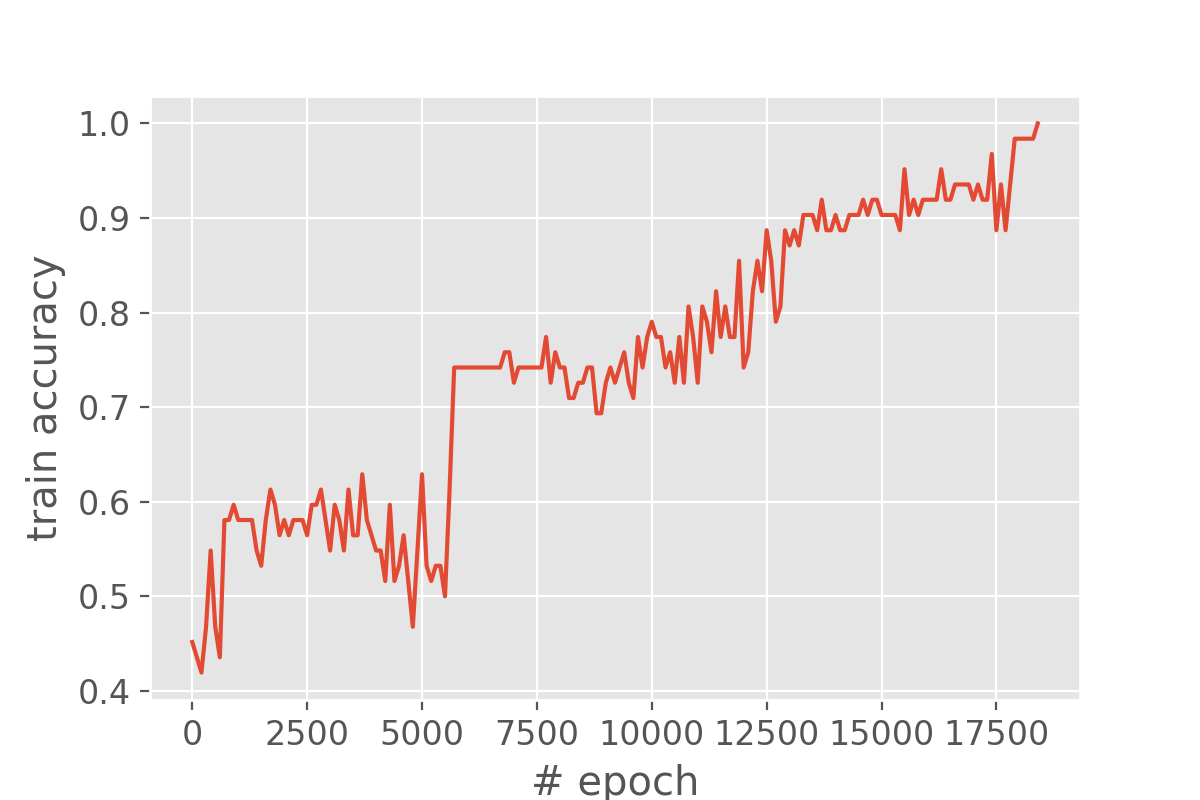
\includegraphics[scale=0.6]{LSTM-128_parity_train_accuracy.png} \par
    \caption{train accuracy}
\end{subfigure}%
\begin{subfigure}{.5\textwidth}
    \centering
    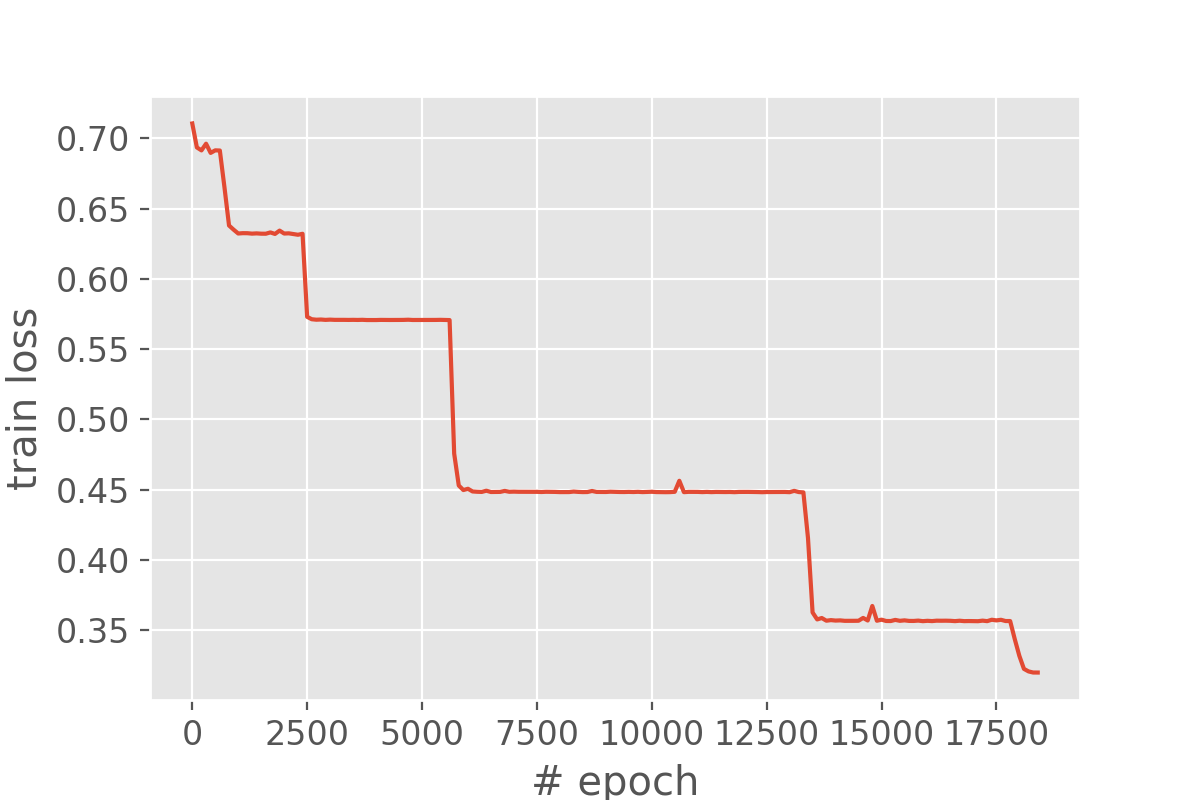
\includegraphics[scale=0.6]{LSTM-128_parity_train_loss.png} \par
    \caption{train loss}
\end{subfigure}
\caption{LSTM-128 training with the learning rate of 0.0005}
\label{fig:lstm128-training}
\end{figure}

%==============================================================================%
\newpage
\begin{task}{2.2} 
\texttt{driver\_parity.py} also evaluates your trained model on binary sequences of length 0 to 20 and saves a corresponding plot of accuracy vs.~length. Include this plot in your write-up and describe the trend you observe. Why might the model behave this way?
\end{task}

The model validation accuracy is shown in Figure \ref{fig:lstm128-generalization}. The model seemed to perform very well with strings of length less than or equal to 5. However, its performance started to degrade significantly with longer sequences until reaching the same accuracy as random guess with sequences longer than 13. The perfect accuracies for short sequences and the fact that we only trained the model with such sequences might imply over-fitting. One possible reason might be that the training data did not represent the population. Another reason might be the high complexity of the model.

\begin{figure}[H]
    \centering
    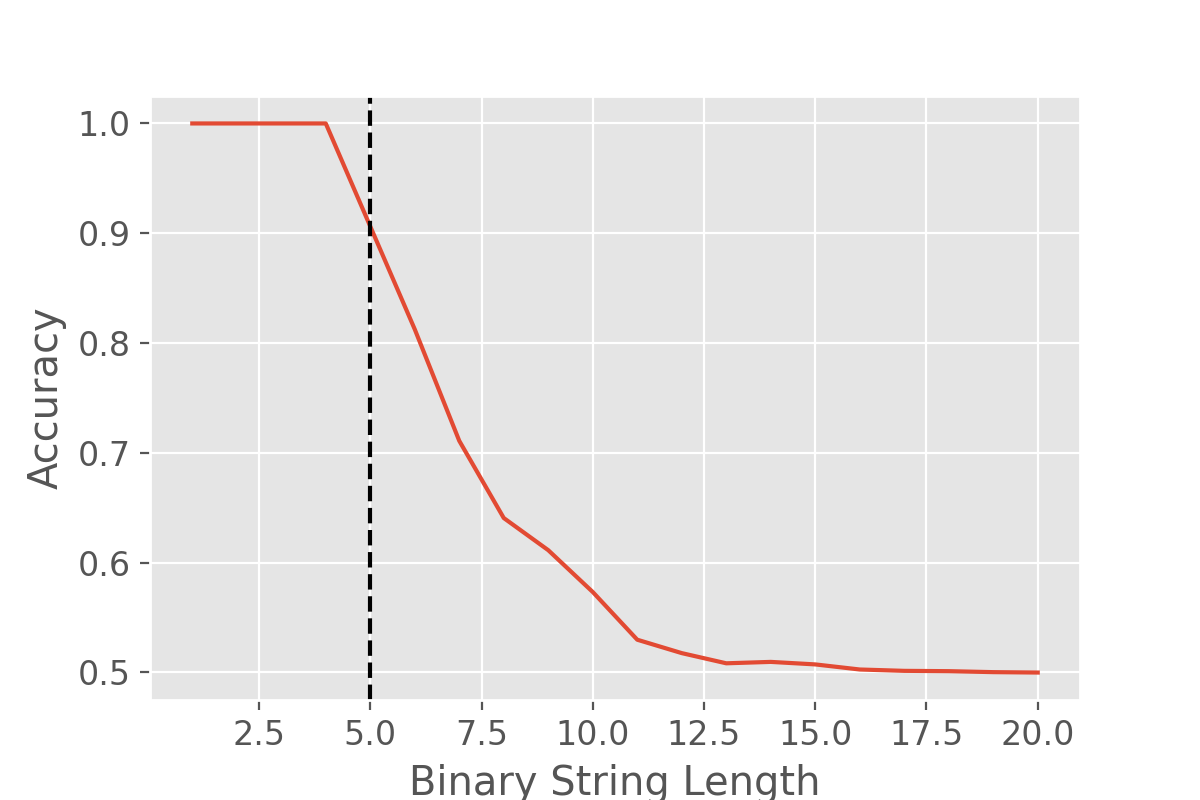
\includegraphics[scale=0.5]{LSTM-64_parity_generalization.png} \par
    \caption{LSTM-128 parity generalization}
    \label{fig:lstm128-generalization}
\end{figure}

%==============================================================================%
\newpage
\begin{task}{2.3} 
We know from 1.1 that even a univariate LSTM (one with a scalar hidden state) can theoretically solve this problem. Run a few (3-4) experiments with different hidden state sizes, what is the smallest size for which you can still train to fit this dataset? Feel free to adjust any of the hyper-parameters in the optimization in the \texttt{train\_model} function if you want. Describe any trends you saw in training or the generalization experiment as you reduced the model capacity.
\end{task}

Models with hidden dimension of 64, 16, 4, and 2 were experimented with training for as many as 80000 epochs at the learning rate of 0.0005, as shown in the figure \ref{fig:lstm64-training}, \ref{fig:lstm16-training}, \ref{fig:lstm4-training}, and \ref{fig:lstm2-80000-training}. Unlike theory suggests, the smallest size LSTM that can fit the data set seemed to be 4. 

The model with 2 hidden units seemed not to improve much after reaching about 0.98 training accuracy. However, figure \ref{fig:lstm2-80000-training} shows that it took about 60000 epochs before a surge in accuracy occurs, which implies that the model might be able to escape the plateau if it is given more training time. Another 2-hidden-unit model was trained with 200000 epochs. As demonstrated by figure \ref{fig:lstm2-200000-training}, the performance was even worse than the one trained with 80000 epochs, possibly due to random initialization.

\begin{figure}[H]
\centering
\begin{subfigure}{.5\textwidth}
    \centering
    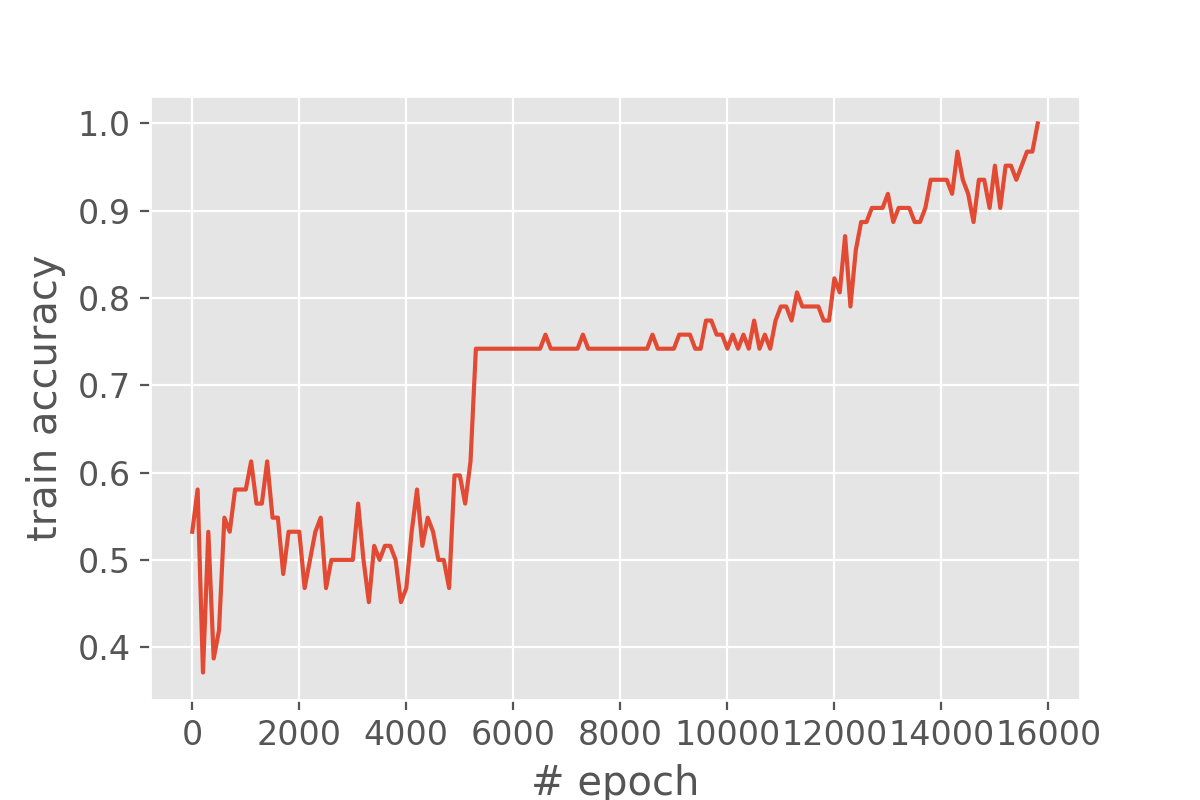
\includegraphics[scale=0.6]{LSTM-64_parity_train_accuracy.png} \par
    \caption{train accuracy}
\end{subfigure}%
\begin{subfigure}{.5\textwidth}
    \centering
    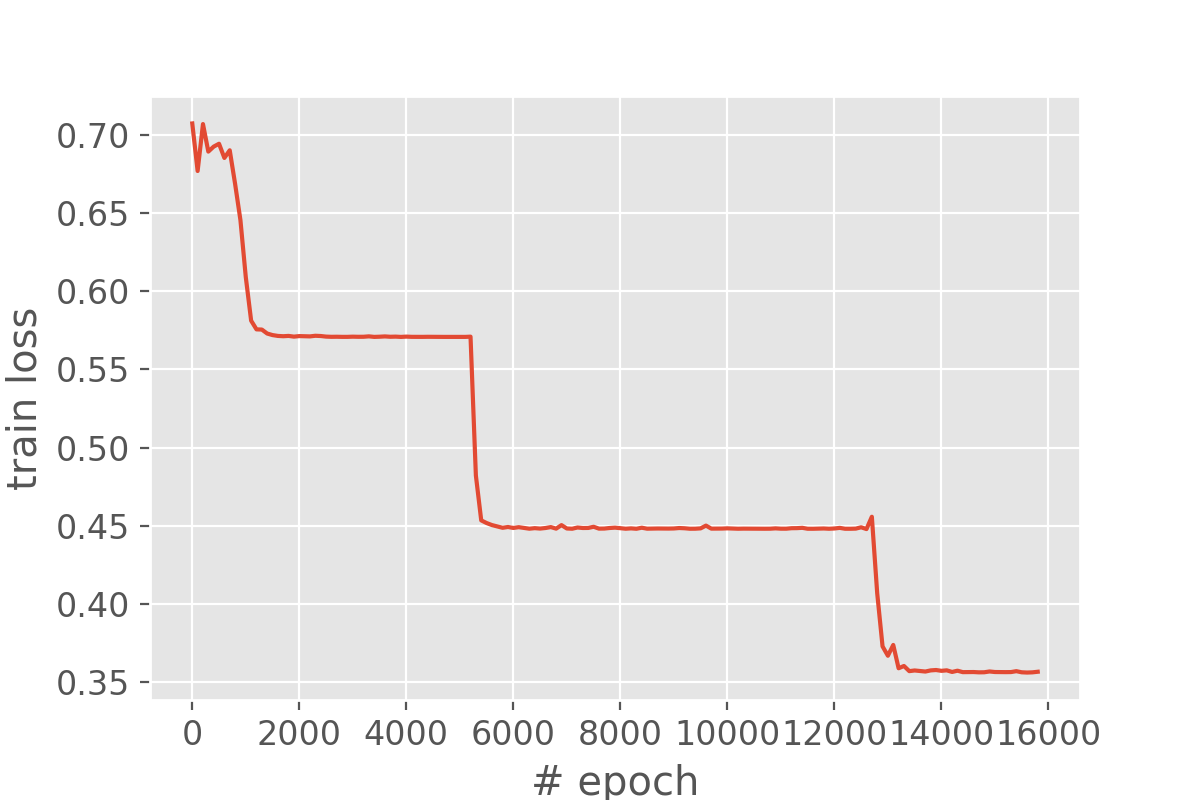
\includegraphics[scale=0.6]{LSTM-64_parity_train_loss.png} \par
    \caption{train loss}
\end{subfigure}
\caption{LSTM-64 training with the learning rate of 0.0005}
\label{fig:lstm64-training}
\end{figure}

\begin{figure}[H]
\centering
\begin{subfigure}{.5\textwidth}
    \centering
    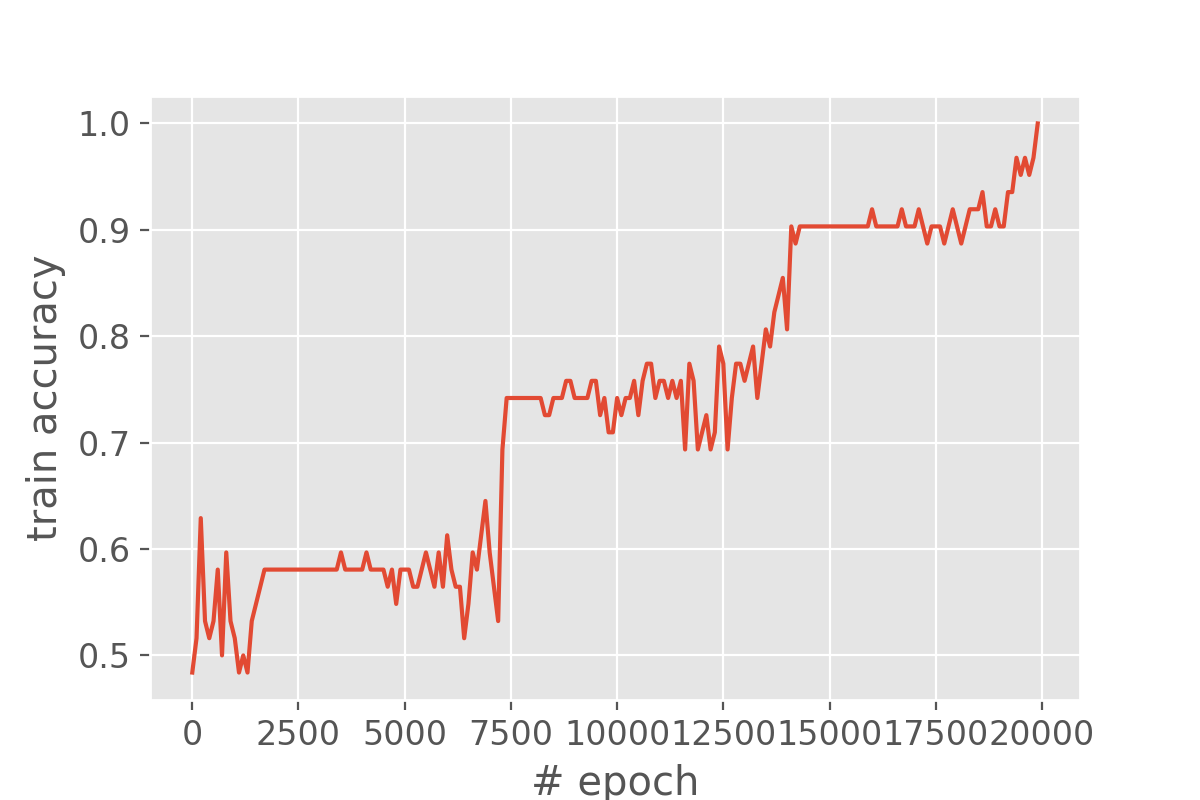
\includegraphics[scale=0.6]{LSTM-16_parity_train_accuracy.png} \par
    \caption{train accuracy}
\end{subfigure}%
\begin{subfigure}{.5\textwidth}
    \centering
    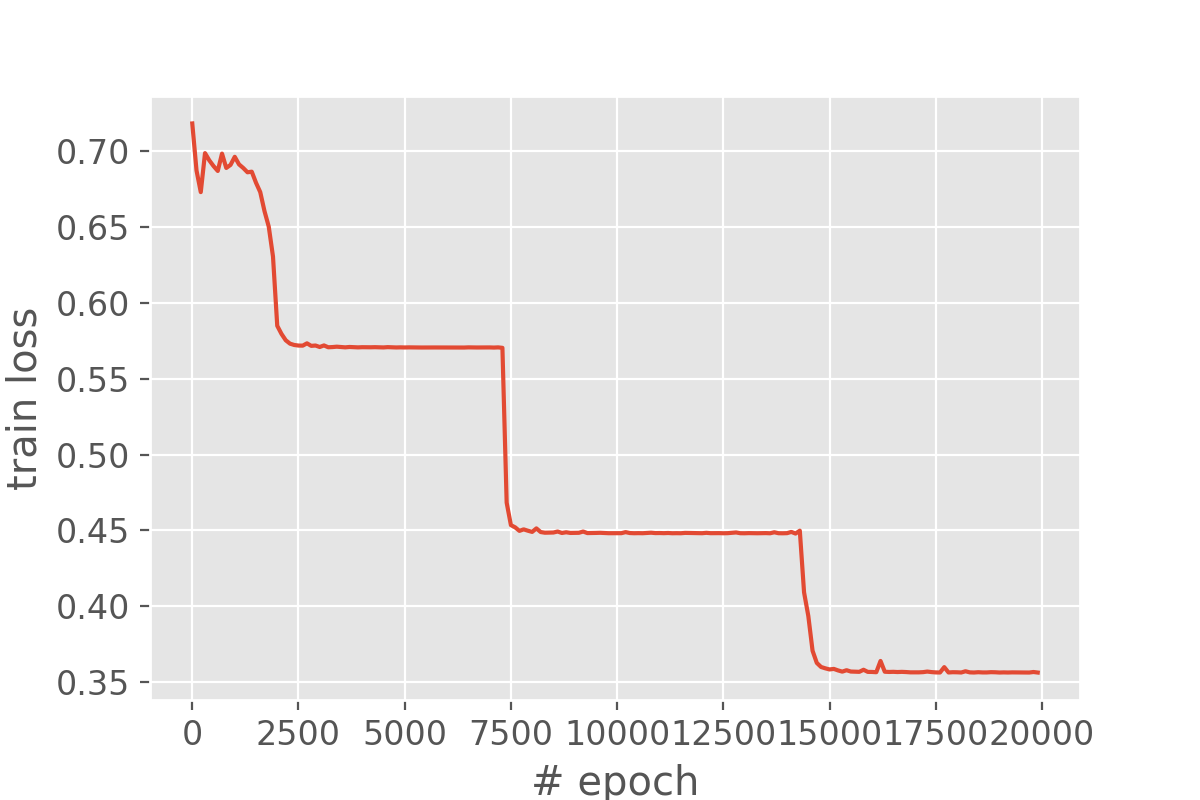
\includegraphics[scale=0.6]{LSTM-16_parity_train_loss.png} \par
    \caption{train loss}
\end{subfigure}
\caption{LSTM-16 training with the learning rate of 0.0005}
\label{fig:lstm16-training}
\end{figure}

\begin{figure}[H]
\centering
\begin{subfigure}{.5\textwidth}
    \centering
    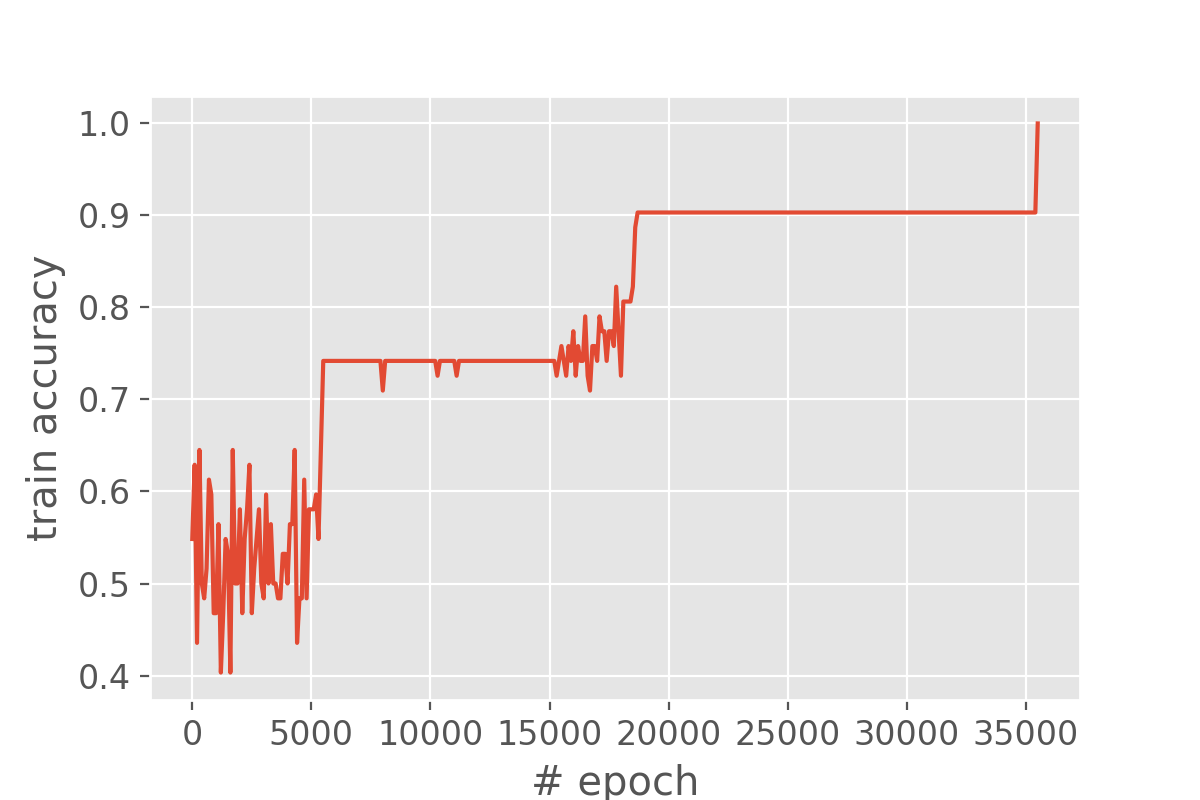
\includegraphics[scale=0.6]{LSTM-4_parity_train_accuracy.png} \par
    \caption{train accuracy}
\end{subfigure}%
\begin{subfigure}{.5\textwidth}
    \centering
    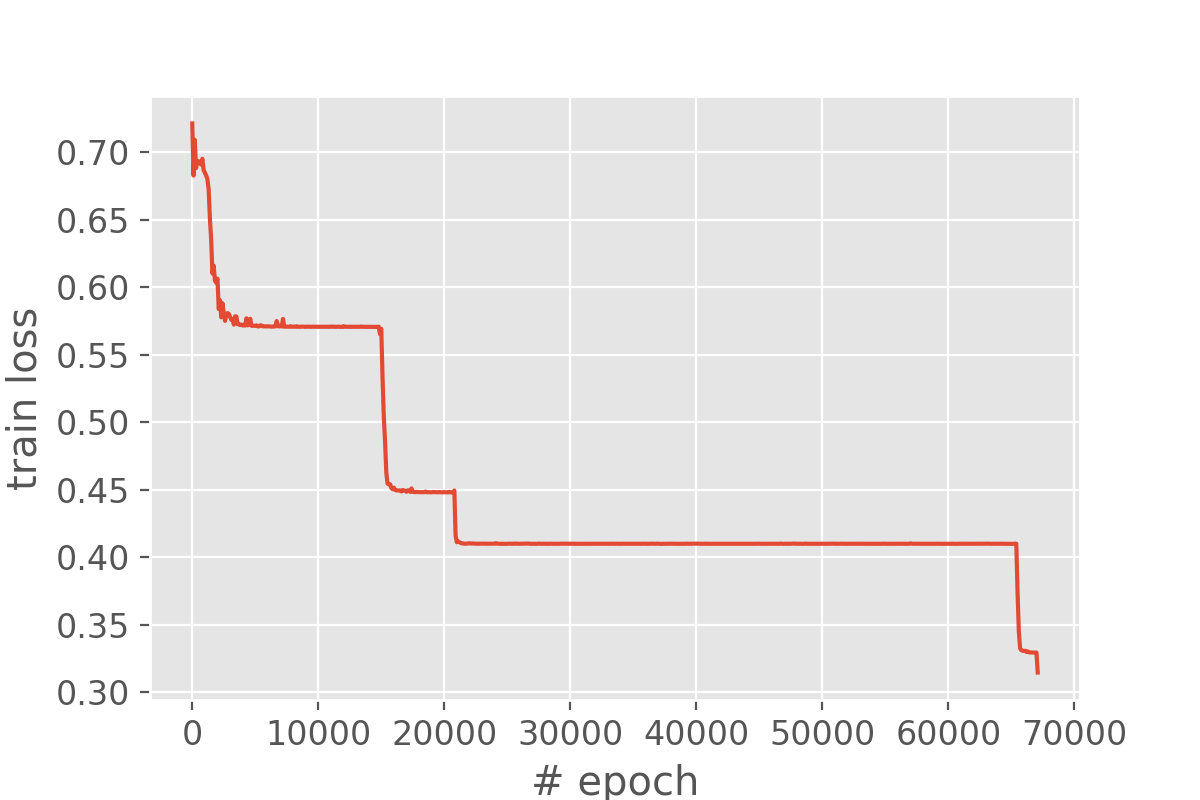
\includegraphics[scale=0.6]{LSTM-4_parity_train_loss.png} \par
    \caption{train loss}
\end{subfigure}
\caption{LSTM-4 training with the learning rate of 0.0005}
\label{fig:lstm4-training}
\end{figure}

\begin{figure}[H]
\centering
\begin{subfigure}{.5\textwidth}
    \centering
    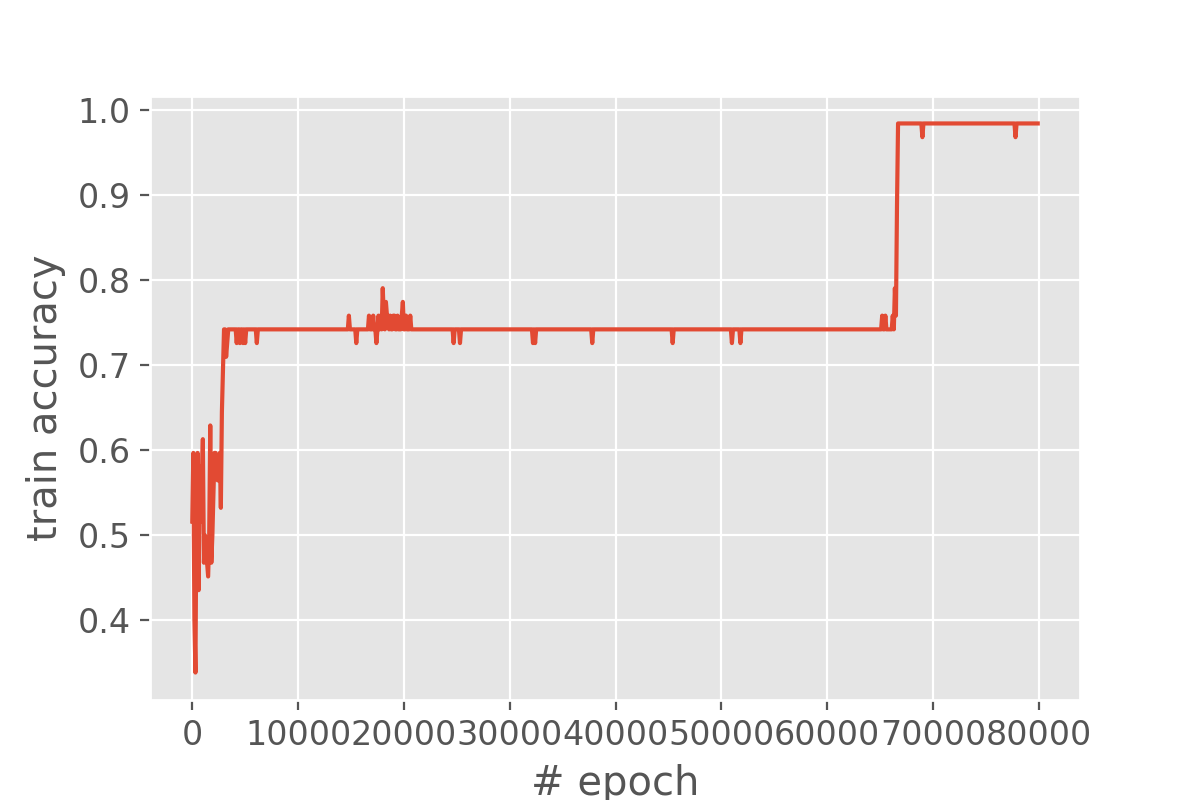
\includegraphics[scale=0.6]{LSTM-2-80000_parity_train_accuracy.png} \par
    \caption{train accuracy}
\end{subfigure}%
\begin{subfigure}{.5\textwidth}
    \centering
    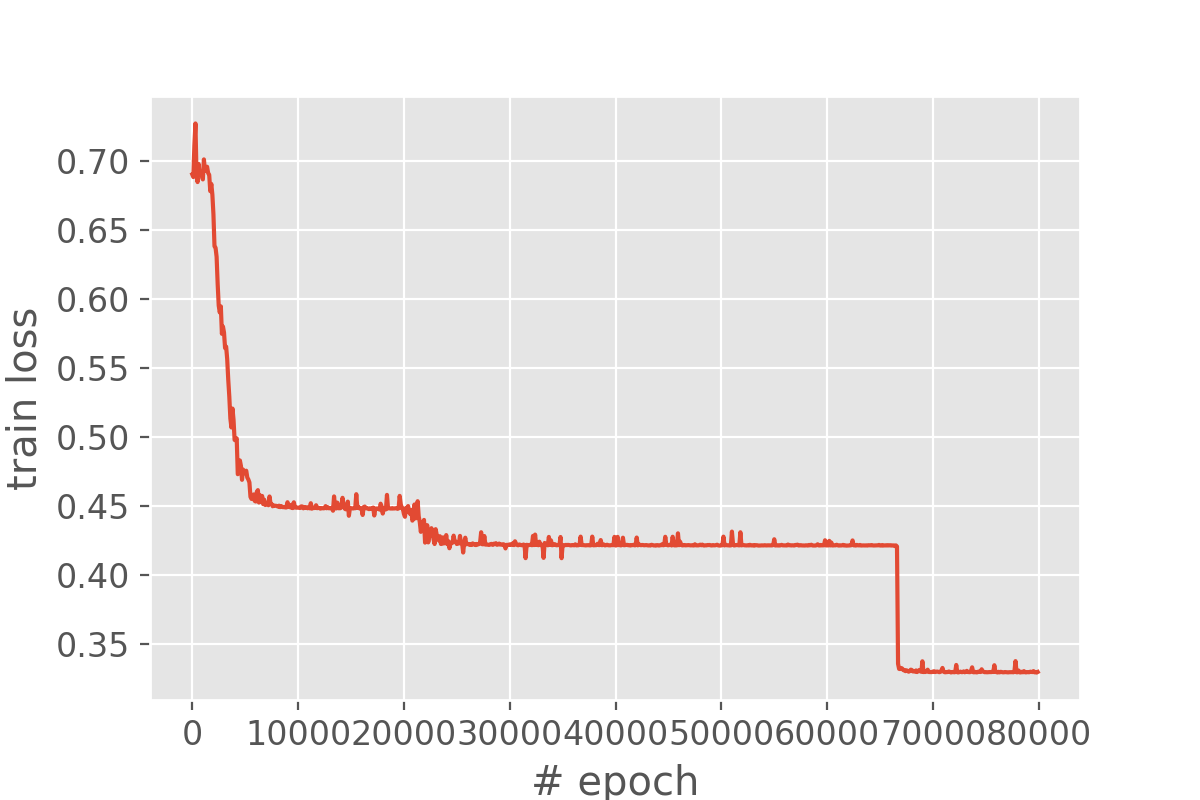
\includegraphics[scale=0.6]{LSTM-2-80000_parity_train_loss.png} \par
    \caption{train loss}
\end{subfigure}
\caption{LSTM-2 training with 80000 epochs}
\label{fig:lstm2-80000-training}
\end{figure}

\begin{figure}[H]
\centering
\begin{subfigure}{.5\textwidth}
    \centering
    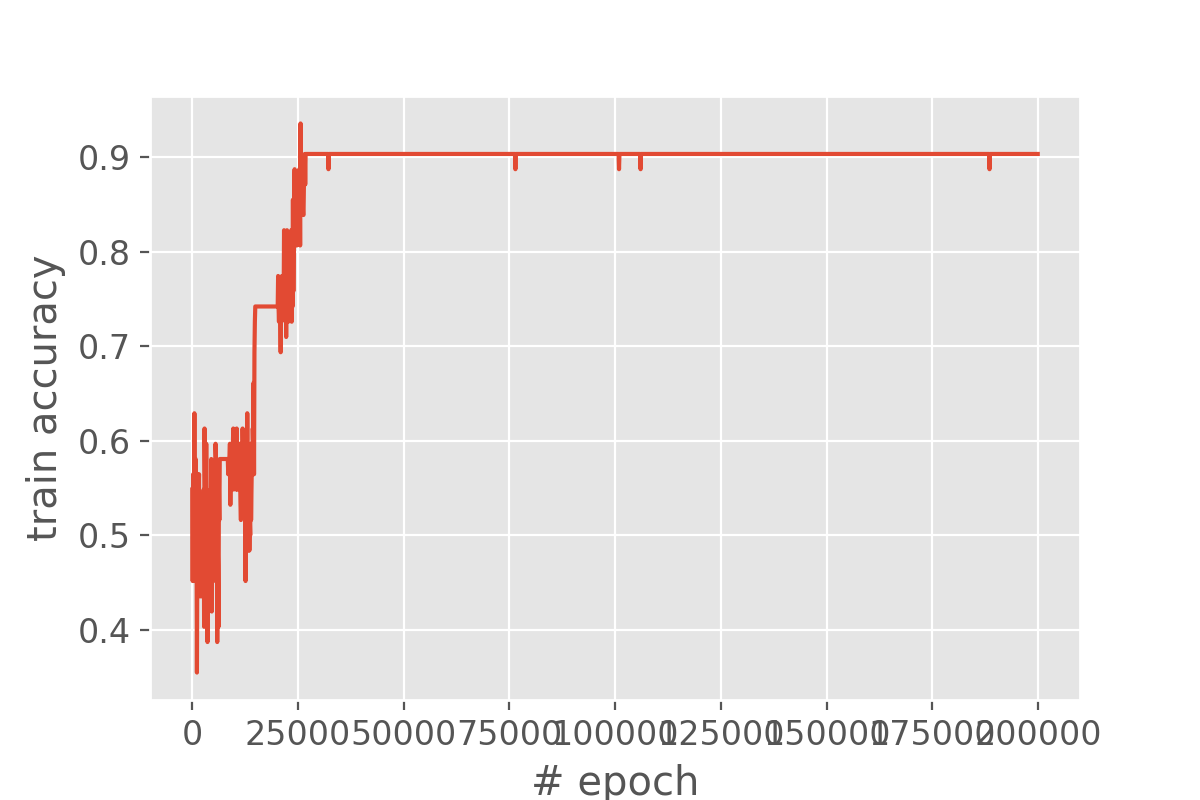
\includegraphics[scale=0.6]{LSTM-2-200000_parity_train_accuracy.png} \par
    \caption{train accuracy}
\end{subfigure}%
\begin{subfigure}{.5\textwidth}
    \centering
    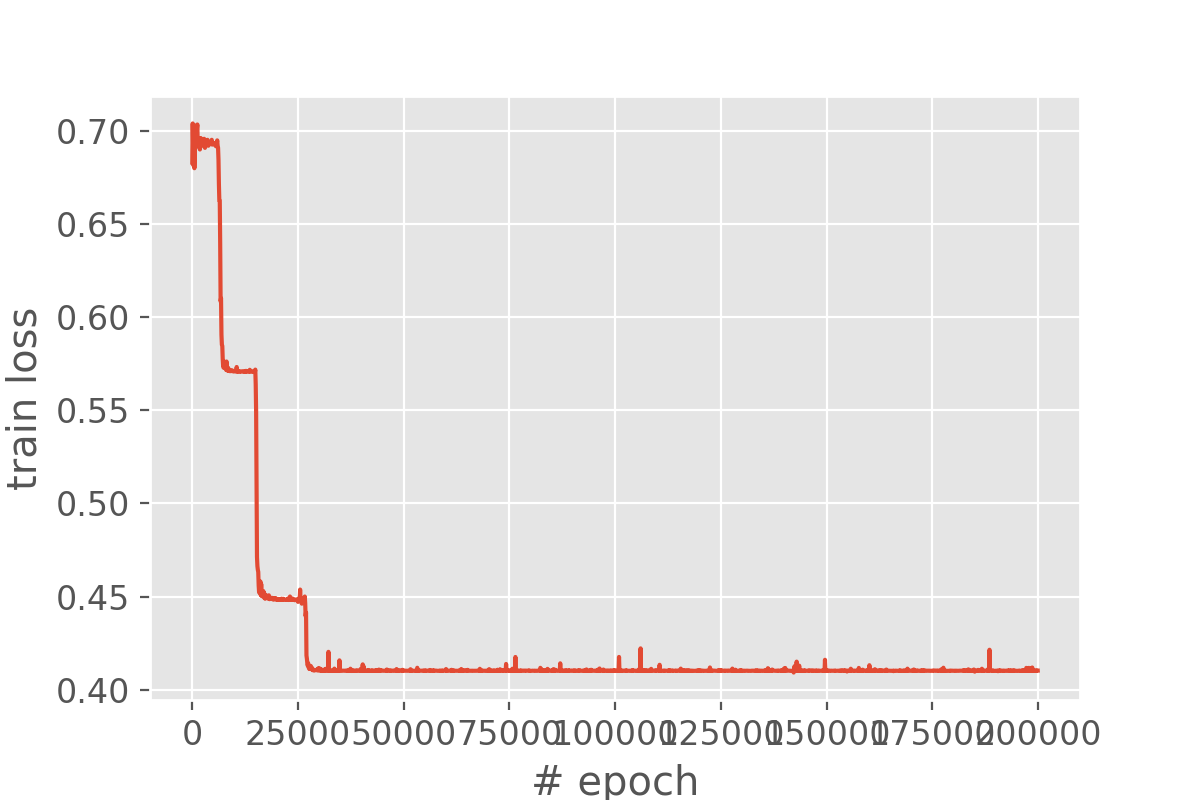
\includegraphics[scale=0.6]{LSTM-2-200000_parity_train_loss.png} \par
    \caption{train loss}
\end{subfigure}
\caption{LSTM-2 training with 200000 epochs}
\label{fig:lstm2-200000-training}
\end{figure}


%==============================================================================%
\newpage
\begin{task}{2.4} 
It has been demonstrated that vanilla RNNs have a hard time learning to classify whether a string was generated by an ERG or not. LSTMs on the other hand seem to work fine. Based on the structure of the problem and what you know about recurrent networks, why might this be the case? 
\end{task}

The advantage of LSTM or other networks based on the gated recurrent unit is the ability to forget old state that was already "learned" by the model. This makes LSTM insusceptible to vanishing or exploding gradients. ERG strings with k = 4 have the lengths of at least 24, which are long enough to cause vanishing or exploding gradients. This might be the reason why RNN could not learn much, whereas LSTM performed quite well in this task.
%==============================================================================%
\newpage
\begin{task}{3.1} 
The first step for any machine learning problem is to get familiar with the dataset. Read through random samples of the dataset and summarize what topics it seems to cover. Also look at the relationship between words and part-of-speech tags -- what text preprocessing would be appropriate or inappropriate for this dataset? Produce a histogram of part-of-speech tags in the dataset -- is it balanced between all tags? What word-level accuracy would a simple baseline that  picked the majority label achieve?
\end{task}

The texts in the data seem to cover from and wide range of topics from macro ones such as economics and politics to daily life stuff like service complaints. For text preprocessing, lower casing might be appropriate because it does change the grammatical meaning of words, but helps eliminate duplicates. On the other hand, removing stopwords might lose some valuable information about the surrounding words. For example, 'the' and 'a' are usually followed by a noun phrase. Likewise, removing punctuations is not a good idea. Punctuations informs the model about the start and end of sentences, which are important for guessing grammatical roles of words. Last, emojis can be useful for the model too. For example, in the sentence "I \heart\ this song so much.", \heart\ is used as a verb. If the model could recognize \heart\ as a verb, the predictions for the following words would be more certain.

As shown by Figure \ref{fig:tag-dist}, the distribution of tags is not uniform. The data set has 34781 nouns but only 6707 interjection. If we guess every word as a noun, we get an accuracy of 17\%.

\begin{figure}[H]
    \centering
    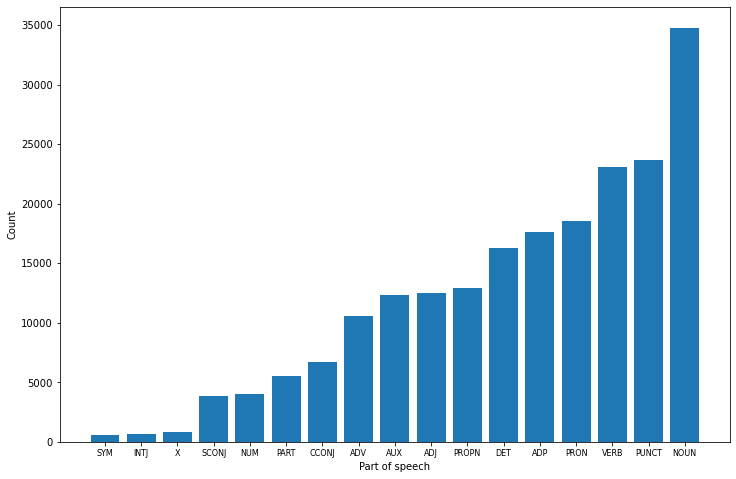
\includegraphics[scale=0.5]{tags_dist.png} \par
    \caption{Tags distribution}
    \label{fig:tag-dist}
\end{figure}


%==============================================================================%
\newpage
\begin{task}{3.2} 
Create a file \texttt{driver\_udpos.py} that implements and trains a bidirectional LSTM model on this dataset with cross entropy loss. The BiLSTM should predict an output distribution over the POS tags for each token in a sentence. In your written report, produce a graph of training and validation loss over the course of training. Your model should be able to achieve $>70\%$ per-word accuracy fairly easily. \\[5pt] 

To achieve stronger performance, you will likely need to tune hyper-parameters or model architecture to achieve lower validation loss. Using pretrained word vectors will likely help as well. You may also wish to employ early-stopping -- regularly saving the weights of your model during training and then selecting the saved model with the lowest validation loss. In your report, describe any impactful decisions during this process. Importantly -- \texttt{DO NOT EVALUATE ON TEST DURING THIS TUNING PROCESS}.\\[5pt]

Once you are done finetuning, evaluate on the test split of the data and report the per-word accuracy. 
\end{task}

%==============================================================================%
\begin{task}{3.3} 
Implement a function \texttt{tag\_sentence(sentence, model)} that processes an input sentence (a string) into a sequence of POS tokens. This will require you to tokenize/numeralize the sentence, pass it through your network, and then print the result. Use this function to tag the following sentences:\\[5pt]

The old man the boat.

The complex houses married and single soldiers and their families.

The man who hunts ducks out on weekends.    
\end{task}

\bibliographystyle{alpha}
\bibliography{mybib}
\end{document}
